\documentclass[11pt]{beamer}

\usetheme{metropolis}

\usepackage{graphicx}
\usepackage{physics}
\usepackage{adjustbox}
\usepackage{caption}
\usepackage{chemformula}
\usepackage{quoting}
\usepackage[style=chem-angew,backend=bibtex]{biblatex}
\bibliography{references}
%
% Choose how your presentation looks.
%
% For more themes, color themes and font themes, see:
% http://deic.uab.es/~iblanes/beamer_gallery/index_by_theme.html
%
\mode<presentation>
{
  \usetheme{default}      % or try Darmstadt, Madrid, Warsaw, ...
  \usecolortheme{default} % or try albatross, beaver, crane, ...
  \usefonttheme{default}  % or try serif, structurebold, ...
  \setbeamertemplate{navigation symbols}{}
  \setbeamertemplate{caption}[numbered]
  \setbeamerfont{footnote}{size=\tiny}
} 

\usepackage[english]{babel}
\usepackage[utf8]{inputenc}
\graphicspath{{image/}}

\AtBeginSection[]{
\begin{frame}{Outline}
  \tableofcontents[currentsection]
\end{frame}
}

\title{Chapter 4: Chemical Composition}
\institute{Chemistry Department, Cypress College}
\date{Sept 14, 2022}

\begin{document}

\begin{frame}
  \titlepage
\end{frame}

\section{Teaching Philosophy and Week 5 Agenda}

\begin{frame}{Teaching Philosophy}
  \textbf{Humanist-inspired pedagogy:}
  \begin{itemize}
  \item Student-teacher relationship is central
    \begin{itemize}
    \item Mutual respect and growth
    \item ``Unconditional positive regard''
    \item Awareness of the other and their thoughts/emotions
    \item Teacher is coach/supporter/mentor rather than supervisor/boss
    \end{itemize}
  \item Focus on attitude and approach rather than content
  \item Learning to fail
  \item Collaboration rather than competition
  \item Explore and experience something new together, learn about
    chemistry and ourselves
  \end{itemize}
\end{frame}

\begin{frame}{Making the Most of It}

  Questions to consider:
  \begin{itemize}
  \item Why am I taking this course?
  \item What would I like to achieve?
  \item What methods/tools/resources work for me?
  \end{itemize}

  Your feedback, questions, participation are vital:
  \begin{itemize}
  \item Attend lectures and discussions, if possible
  \item Give on-going feedback to instructors through facial expression,
    emojis, chat, email, during office hours etc.
  \item Fill out evaluations
  \item Own your education
  \item Be proactive, do not hesitate to speak up or get help
  \end{itemize}

\end{frame}

\begin{frame}{Lecture and Lab Weekly Agenda}
  \textbf{Lab Section}

  \begin{itemize}
  \item Experiment 2 - Measurements: Temp, Mass, Length, Volume,
    and Density
  \item Demonstration - weighing the scale
  \item Warning - Do not leave therometer touching the
    bottom of beaker when heating the water
  \end{itemize}

  \textbf{Lecture Section}

  \begin{itemize}
  \item Go over homework assignment 2; present your work
    for 1pt EC
  \item Review Ch 4 - Chemical Composition
  \item Homework and quiz 4 released Fri, Sept 23 at 3pm
  \item Homework due Fri, Sept 30 at 11:59pm
  \item Quiz 4 due Mon, Sept 26 at 11:59pm
  \item \textbf{Important Date:} Exam 1 - approx 1.5 hrs
  \end{itemize}
\end{frame}

\section{Percent Composition}

\begin{frame}{Percent Compsition}
  \textbf{Main Takeaway:} Convert the mass of each component
  to a percentage of the total mass

  \begin{equation}
    P_A = \frac{M_A}{M_\text{Tot}} \times 100\%
  \end{equation}

  where $M_\text{Tot}$ is the total mass, $M_A$ is the mass and $P_A$
  is the percent composition for component $A$
\end{frame}

\begin{frame}{Example Problem: Percent Composition}
  Magnetite, Fe$_3$O$_4$, is a mineral containing $72.4\%$ iron. What
  mass of iron is present in an 837g sample of magnetite?

  \begin{align*}
   \onslide<2->{ (837 \text{g magnetite})\frac{72.4 \text{g iron}}{100 \text{g magnetite}}
    = 606 \text{g iron}}
  \end{align*}
  
\end{frame}

\section{The Mole Concept}

\subsection{Determining Empirical and Molecular Formulas}

\begin{frame}{The Mole Concept}
  \begin{center}
    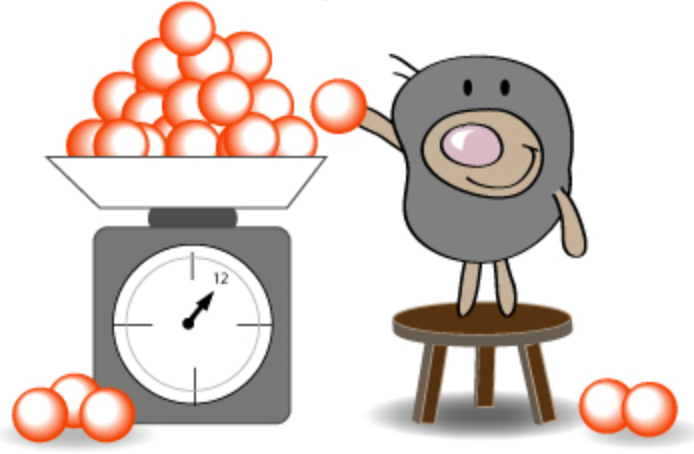
\includegraphics[scale=0.2]{mole}
  \end{center}
  
  \textbf{Q:} What is a mole (mol)?

  \textbf{A:} A mole is measurement of a substance and relates to
  Avogadro's number ($6.022 \times 10^{23}$)

  \textbf{side note:} Mole day is Oct. 23, between 6:02 a.m. and 6:02 p.m
\end{frame}

\begin{frame}{Purpose of the Mole}
  \begin{center}
    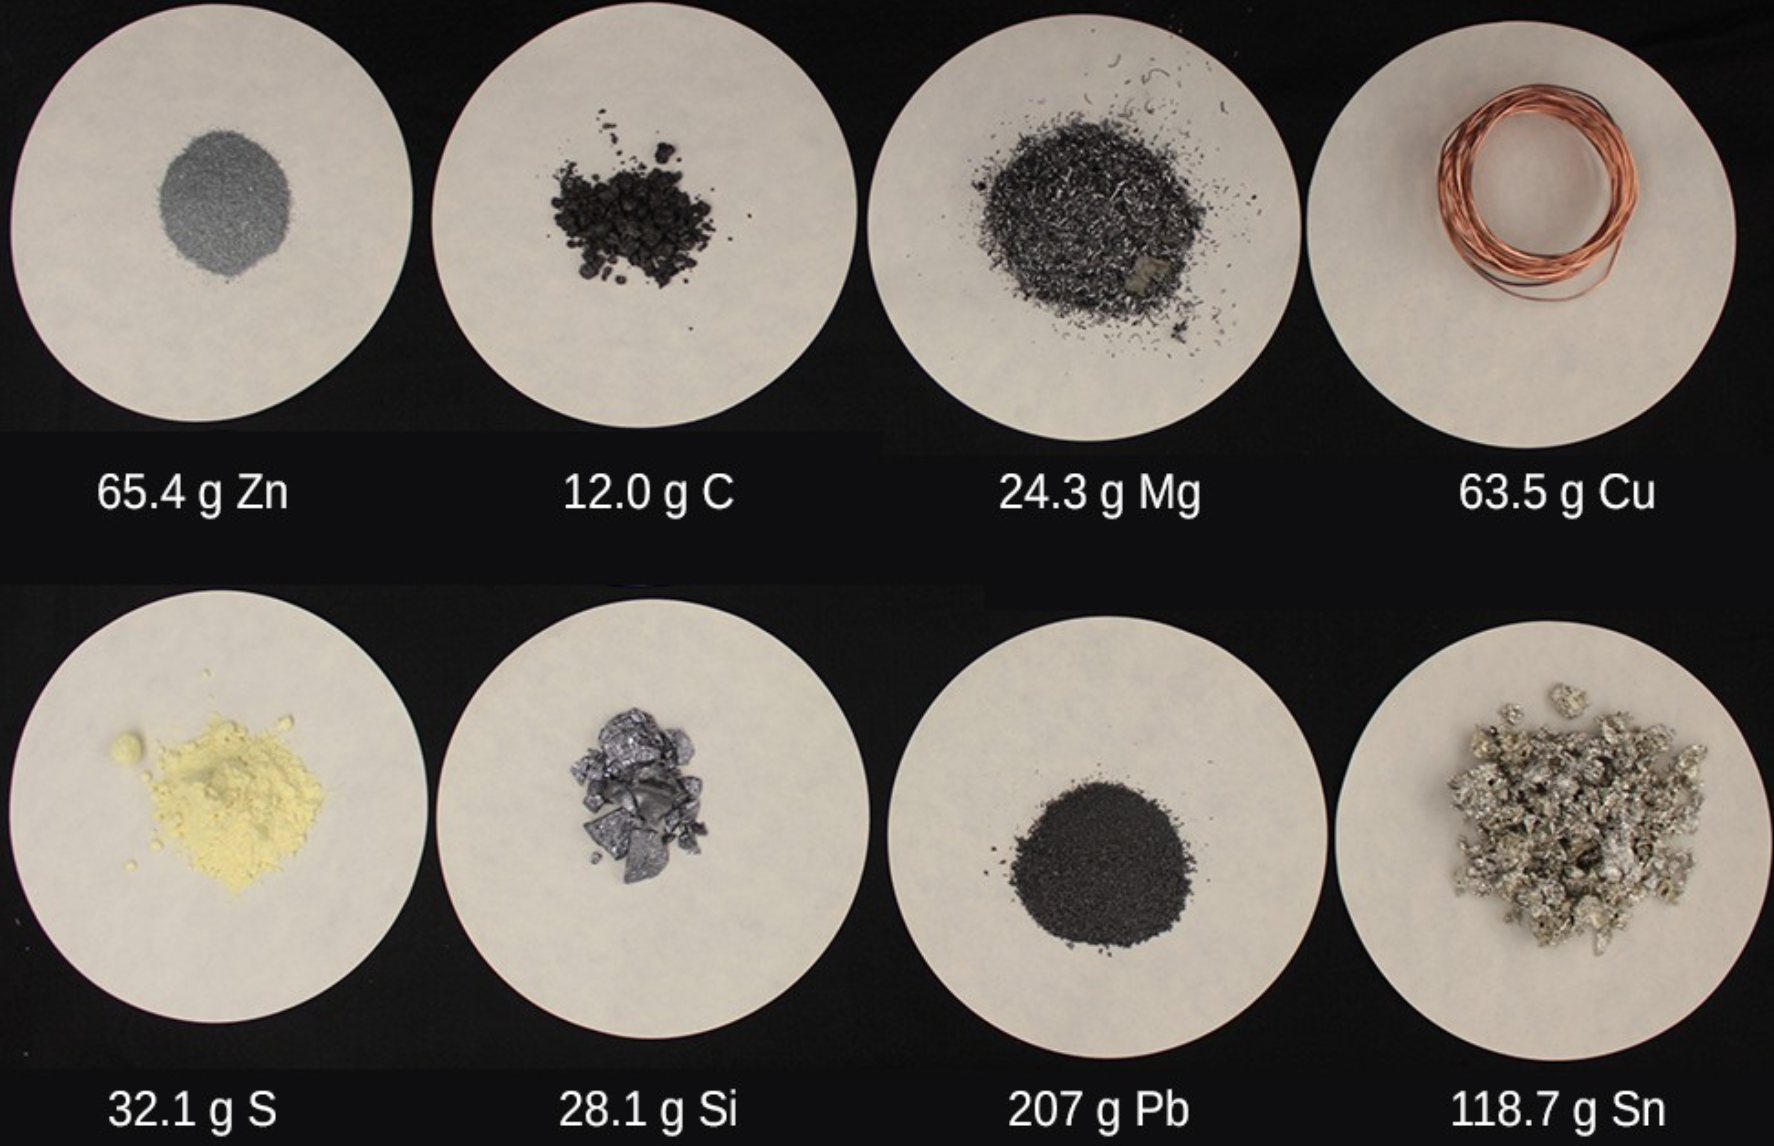
\includegraphics[scale=0.1]{mol_solids}
  \end{center}
  
  \begin{itemize}
  \item Gives a consistent method to convert between atoms/molecules and grams
  \item Convenient way to preform calculations
  \item View the mole (mol) as a unit conversion type approach
  \end{itemize}
\end{frame}

\begin{frame}{Reminder: Periodic Table}
  \begin{center}
    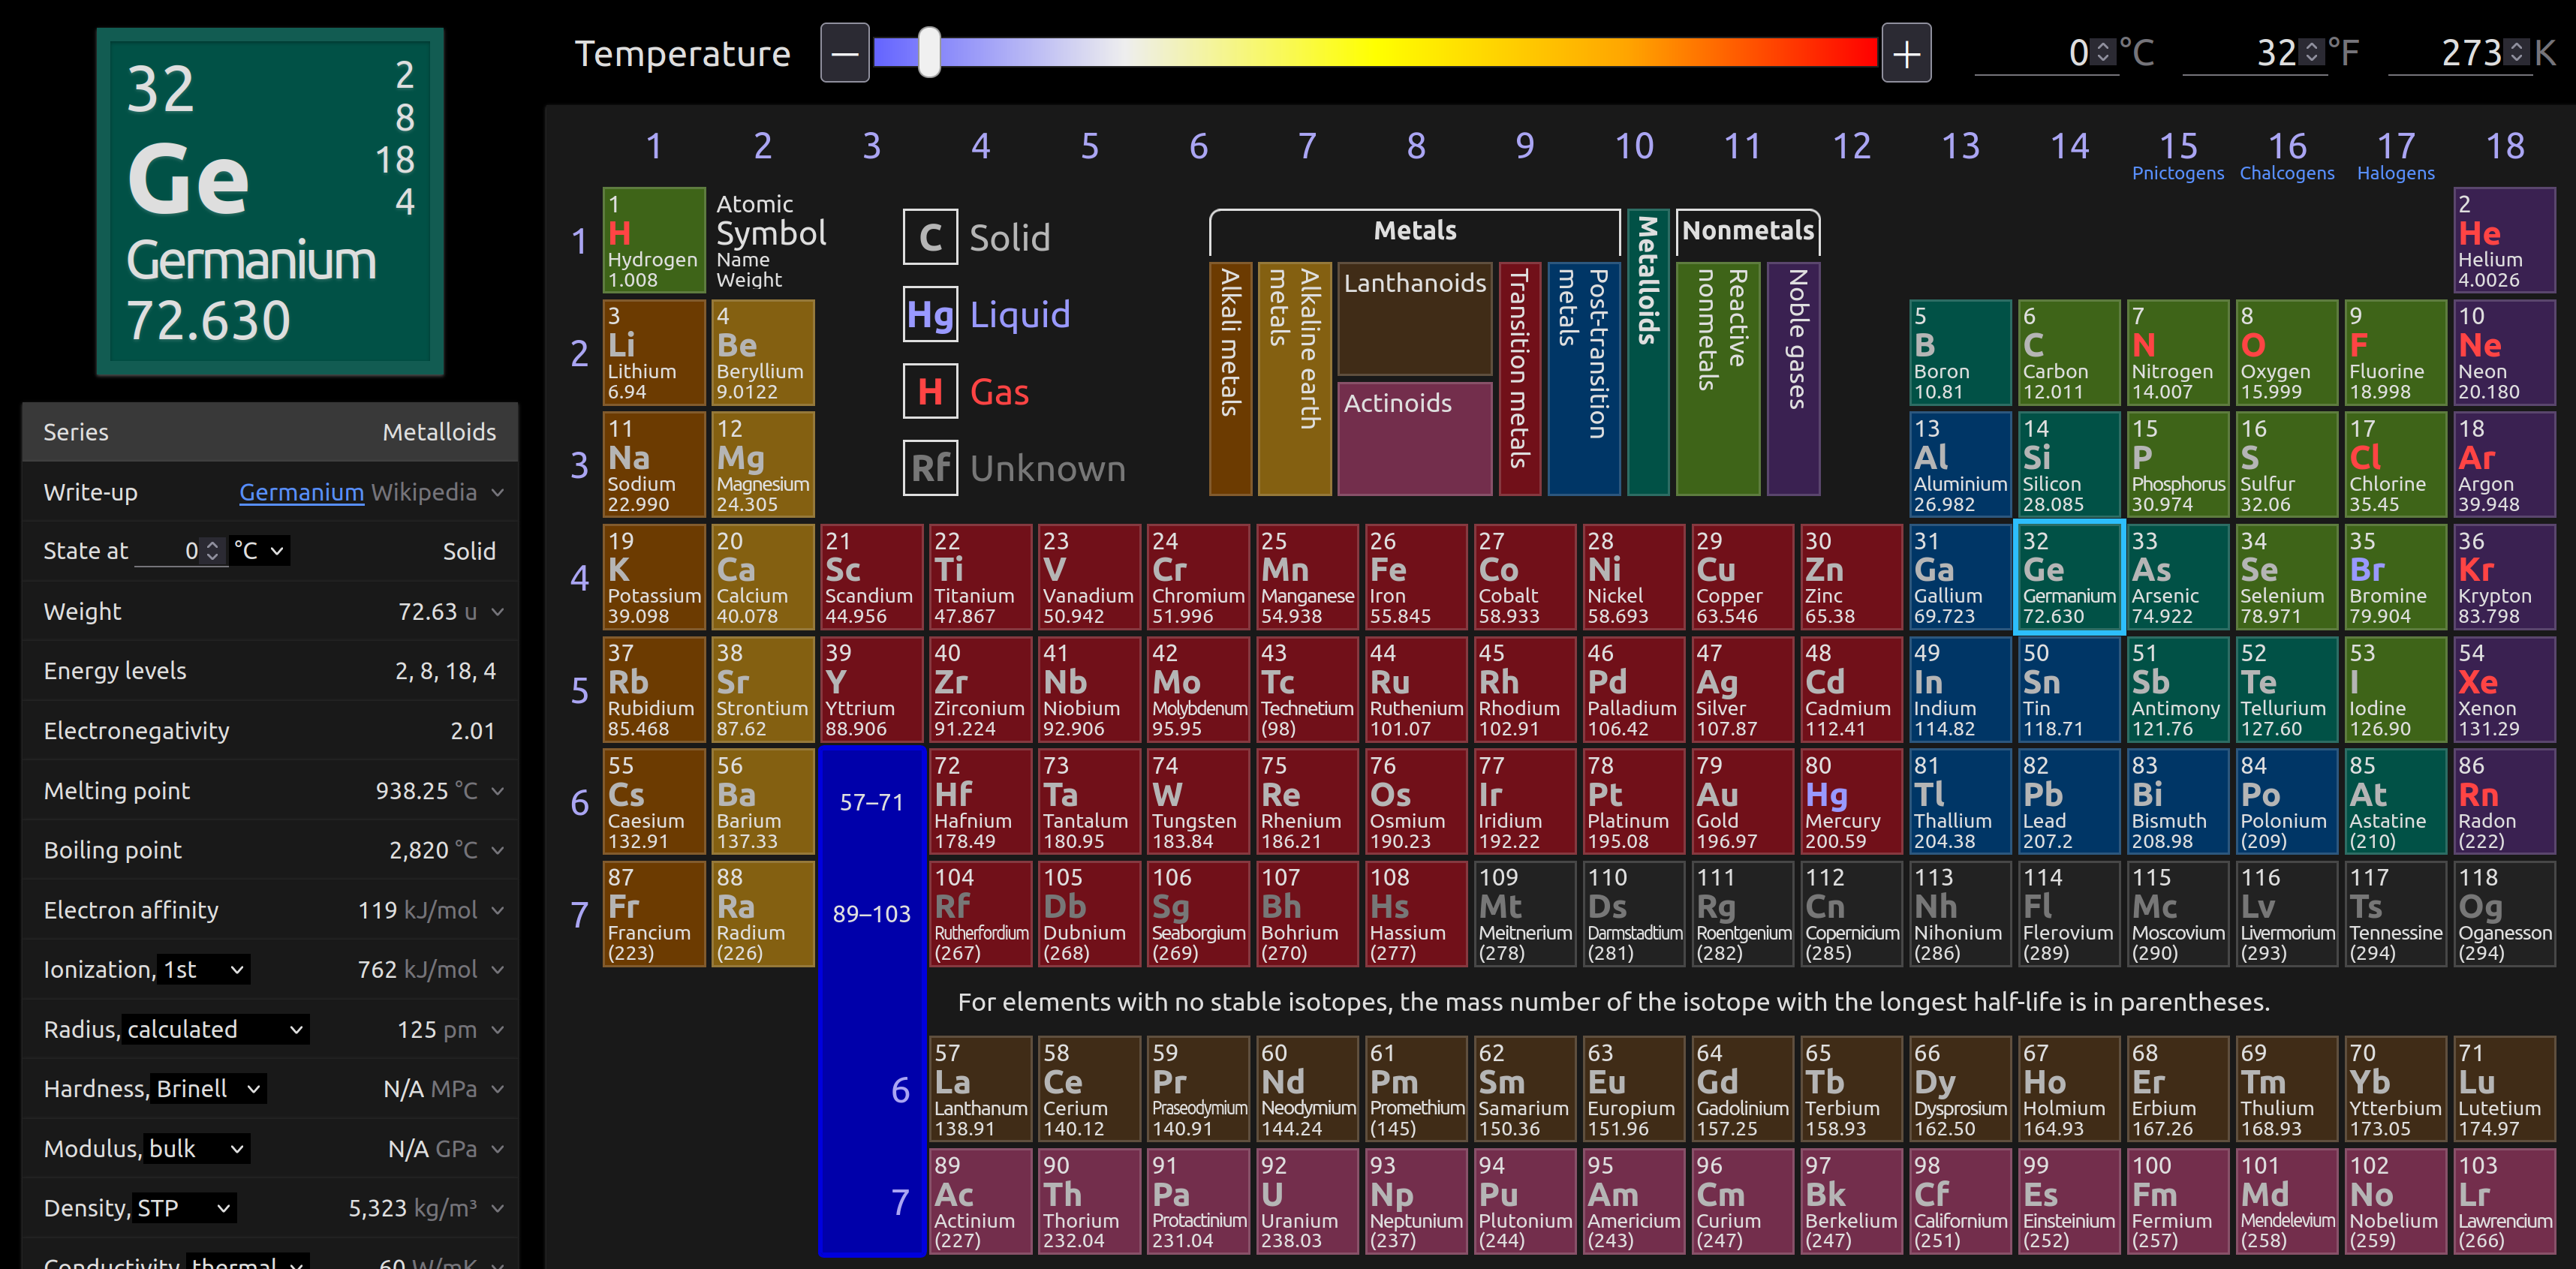
\includegraphics[width=\linewidth]{ptable}
  \end{center}

  \begin{itemize}
  \item Organized based on atomic number,  rel. atomic mass unit,
    and different categories of elements
  \end{itemize}
\end{frame}

\begin{frame}{Relating amu to molar mass}
  \textbf{Atomic Mass Unit} - mass of one atom

  \begin{center}
    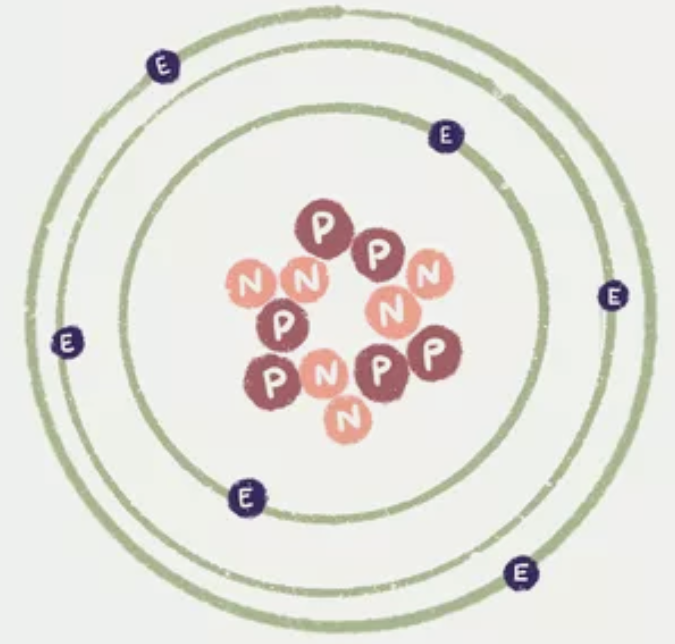
\includegraphics[width=0.25\linewidth]{atomic_mass}
  \end{center}

  \textbf{Molar Mass} - mass of one mole of atoms or molecules

  \textbf{Example:} Determine the molar mass of H$_2$O
  
  \centering
  \onslide<2->{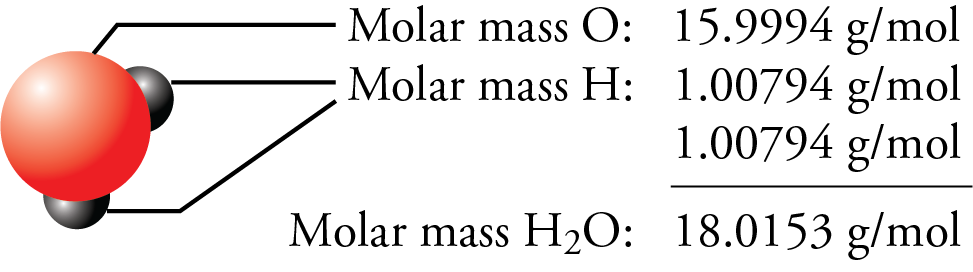
\includegraphics[width=0.7\linewidth]{molar_mass_h2o}}
\end{frame}

\begin{frame}{Periodic Table Revisited}
  \centering
  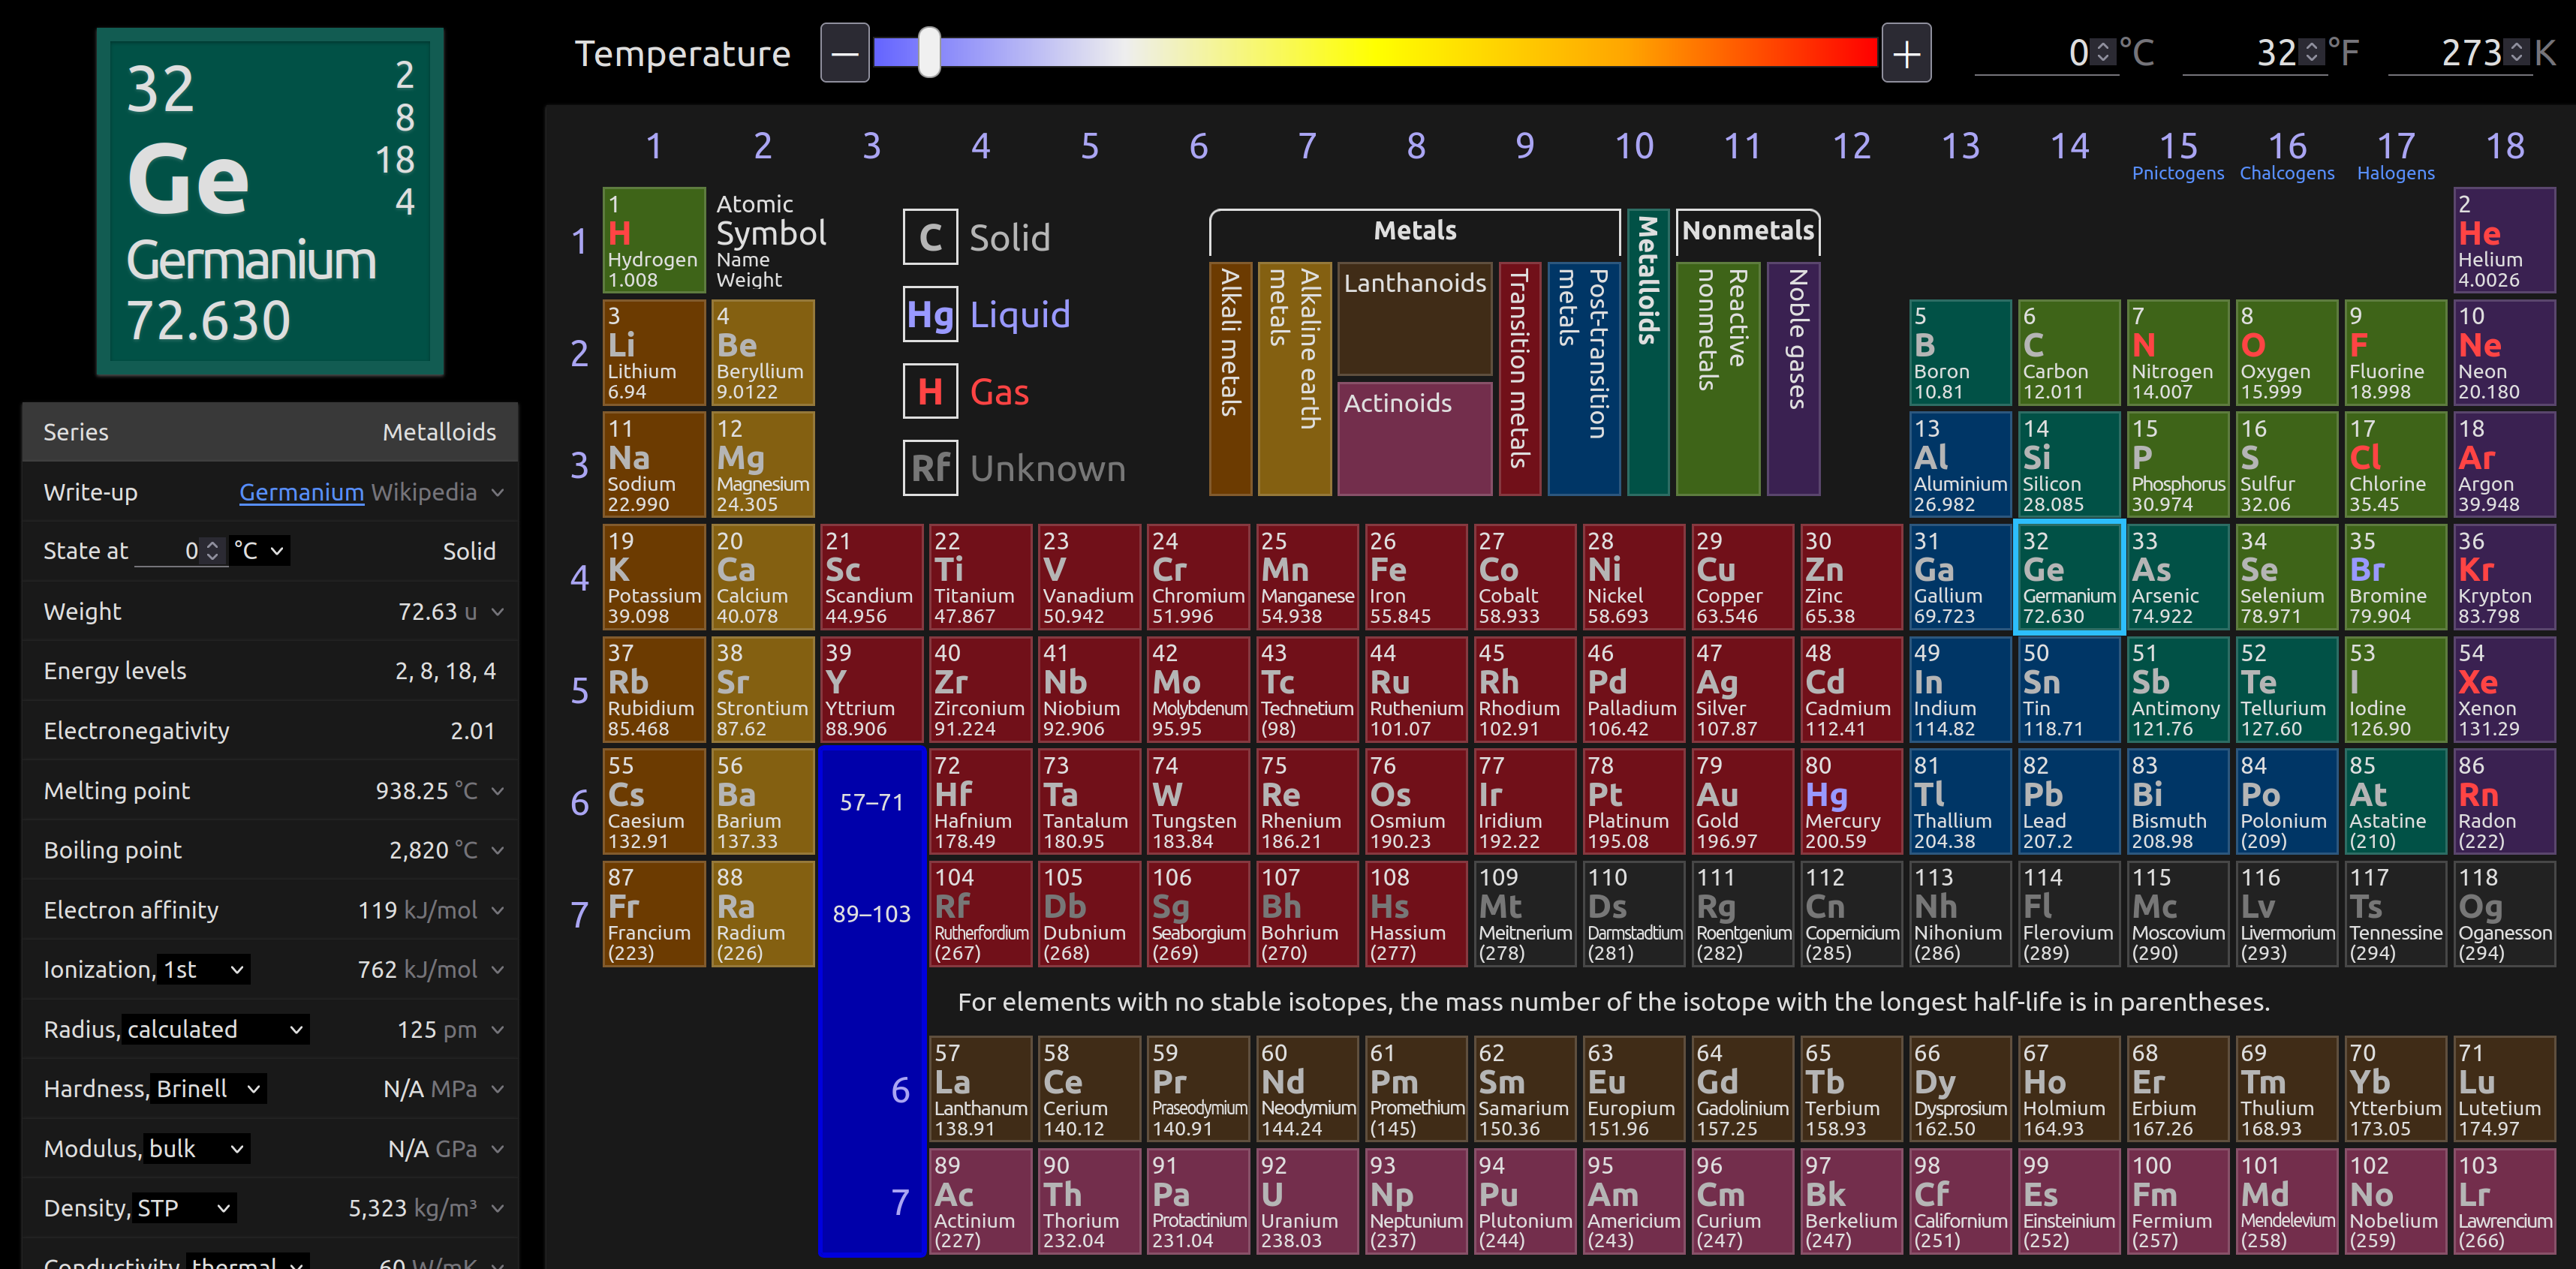
\includegraphics[width=\linewidth]{ptable}

  \textbf{Ge} - 72.630 amu for 1 atom and the molar mass is 72.630 g/mol

  1 amu = $1.66054\times 10^{-24}$ g
\end{frame}

\begin{frame}{Example: Determine the mol of each element within a compound.}
  H$_2$O \onslide<2->{- 2 mols H and 1 mol O}
  
  C$_6$H$_{12}$O$_6$ \onslide<3->{- 6 mols C, 12 mols H, 6 mols O}

  \onslide<3->{\textbf{Practice:} Determine the molar masses}
\end{frame}

\begin{frame}{Example: Mole Connection to Chemical Rxn}
  Zn(s) + 2 HCl(aq) $\rightarrow$ ZnCl$_2$(aq) + H$_2$(g)

  \textbf{Q:} What are the mols of each reagent required to run this reaction?
  And how much mol of each product is produced?

  \onslide<2-> 2 mol Zn(s) and 2 mol HCl(aq) (reagents) produce 1 mol ZnCl$_2$(aq)
  and 1 mol H$_2$(g)
\end{frame}

\begin{frame}{Example: Combine Percent Composition and the Mole}
  Determine the mass percent of each element in Al$_2$(SO$_4$)$_3$.
  \small
  \begin{align*}
    \% \text{ mass of Al} & =
    \onslide<2->{\frac{n\times \text{molar mass Al}}{n \times \text{molar mass of Al$_2$(SO$_4$)$_3$}}
    \times 100\%\\
    & = \frac{2\times 26.98 \text{g}}{342.14 \text{g}} \\
    & = 15.77 \%} \\
    \onslide<3->{\% \text{ mass of S} & =
      \frac{n\times \text{molar mass S}}{n \times \text{molar mass of Al$_2$(SO$_4$)$_3$}}
    \times 100\%\\
    & = \frac{3\times 32.06 \text{g}}{342.14 \text{g}} \\
    & = 28.11 \% \\
    \% \text{ mass of O} & = \frac{n\times \text{molar mass O}}{n \times \text{molar mass of Al$_2$(SO$_4$)$_3$}}
    \times 100\%\\
    & = \frac{12\times 16.00 \text{g}}{342.14 \text{g}} \\
    & = 56.12 \% \\}
  \end{align*} 
\end{frame}

\begin{frame}{Practice: Determine Mass from Moles}
  A friend heats water in a copper kettle and makes a cup of tea. The
  friend adds 0.0120 mol of table sugar (sucrose, C$_{12}$H$_{22}$O$_{11}$).
  What mass of sugar has he added?
  \vfill
\end{frame}

\begin{frame}{Practice: Number of Molecules from Mass}
  A substance named Agorca M5640 is used for concentrating extracted
  copper ore. Its molecular formula is C$_{16}$H$_{25}$NO$_2$. If you have a
  150.0 g sample of Agorca M5640, how many molecules do you have?
  \vfill
\end{frame}

\begin{frame}{Defn: Empirical and Molecular Formulas}
  \textbf{Empirical Formula} - the simplest ratios of atoms in
  a compound; lowest possible ratio

  \textbf{Molecular Formula} - a factor of the empirical formula
\end{frame}

\begin{frame}{Empirical or Molecular Formula?}
  \textbf{Q:} Are the following empirical or molecular formula? If it is a
  molecular formula, then determine the empirical formula.

  \begin{itemize}
  \item H$_2$C$_2$O$_4$
  \item C$_6$H$_3$Cl$_3$
  \item CH$_2$O
  \item HgO
  \end{itemize}
\end{frame}

\begin{frame}{Approach for Empirical/Molecular Problems}
  \begin{itemize}
  \item Convert all elemental masses to mols
  \item Determine the lowest possible ratio
  \item Round to the nearest integer for each element and that
    number is the empirical formula
  \item For molecular formula, use the given experimental molar
    mass and divide by the molar mass of empirical formula. Multiply
    the empirical formula by that ratio.
  \end{itemize}
\end{frame}

\begin{frame}{Practice: Empirical Formula from Percent Composition}
  Determine the empirical formula for the mineral chalcocite, which has
  the percent composition $79.8\%$ Cu and $20.2\%$ S.
  \vfill
\end{frame}

\begin{frame}{Empirical Formula when Ratio is Fractional}
  \begin{itemize}
  \item If the fractional ratio of an element doesn't yield an integer,
    then multiply by a factor e.g. 1/2 multiply by 2, 1/3 multiply by 3, and
    1/4 multiply by 4
  \item When multiplying to an integer, all elements must be multipled by that number
  \end{itemize}
\end{frame}

\begin{frame}{Practice: Determine Empirical Formula}
  The copper mineral azurite has the deep-blue color azure. Azurite contains
  $55.31\%$ copper, $6.97\%$ carbon, $37.14\%$ oxygen, and $0.58\%$ hydrogen. Calculate the
  empirical formula of azurite.
  \vfill
\end{frame}

\begin{frame}{Practice: Determine Molecular Formula}
  The empirical formula for an acid was determined to be HCO$_2$. If the molar mass
  of the acid is determined to be about 90.0g/mol. What is the molecular formula for
  this acid?
  \vfill
\end{frame}

\section{Molarity of Solution}

\subsection{Chemical Composition: Solvent and Solute}

\begin{frame}{Defn: Solvent and Solute}
  \begin{center}
    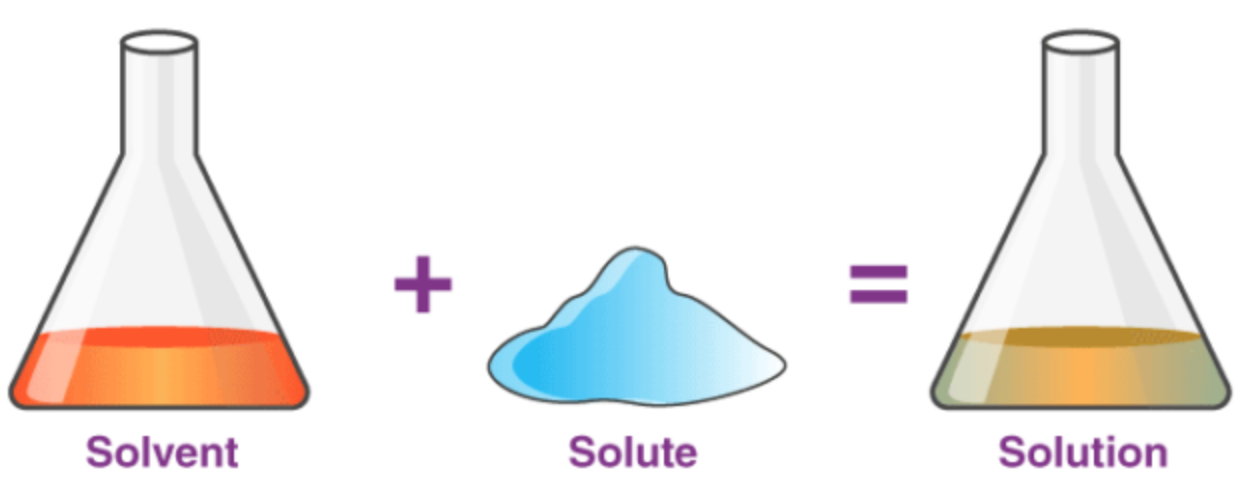
\includegraphics[width=0.75\linewidth]{solut_solv.png}
  \end{center}

  \textbf{Solute} - a substance (solid, liquid, or gas) dissolved in
  a solvent

  \textbf{Solvent} - the material (liquid or gas) that dissolves the
  solute
\end{frame}

\subsection{Concentrations and Dilutions}

\begin{frame}{Molarity - Concentration of Solution}
  \textbf{Definition of Molarity}
  \begin{align}
    M = \frac{n_\text{solute}}{V}
  \end{align}

  where $M$ is molarity, $n_\text{solute}$ is the mols of solute, and $V$ is volume in L

  \textbf{Q:} What is the units for molarity $M$?
\end{frame}

\begin{frame}{Example: Preparing NaCl Solution}
  A solution is prepared from 17.0g of NaCl dissolved in sufficient water to
  give 150.0mL of solution. What is the molarity of the solution? (The molar mass
  of NaCl is 58.44 g/mol.)

  \textbf{Determine} what is given and the question is being asked.
  
  \begin{align*}
    \onslide<2->{n_\text{NaCl} = & 17.0 \text{g NaCl} \times \frac{1 \text{mol NaCl}}{58.44 \text{g NaCl}} \\
    = & 0.2908967 \text{mol NaCl}} \\
    \onslide<3->{V = & 150.0 \text{mL} \times \frac{1\text{L}}{1000\text{mL}}}
  \end{align*}
  \vfill
\end{frame}

\begin{frame}{Practice: Molarity}
  A solution of copper(II) acetate %Cu(CH$_3$CO$_2$)_2$%
  is used as a green dye for textiles. We want to prepare a 0.150$M$ solution of
  copper(II) acetate, starting with 40.0g of the solute. What should be the total
  volume of the solution? (The molar mass of copper(II) acetate is 181.6g/mol.)
  \vfill
\end{frame}

\begin{frame}{Diluting Solutions}
  \begin{center}
    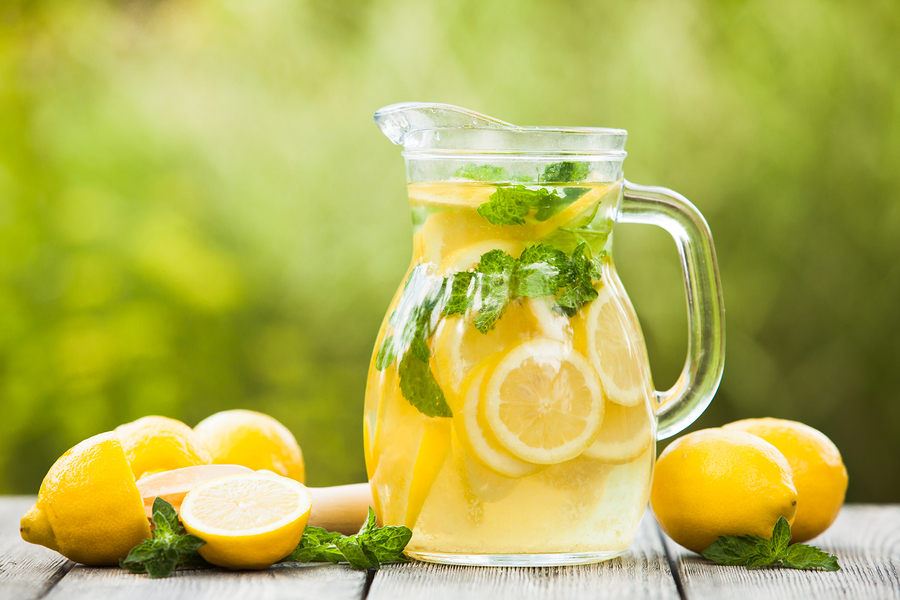
\includegraphics[width=0.4\linewidth]{lemonade}
  \end{center}
  
  Dilution is the process that makes a solution less concentrated. Example is
  lemonade tasting too sweet.

  \textbf{Q:} For given concentrated solution at molarity $M_1$ and a given volume $V_1$, does
  diluting the solution to a new concentration $M_2$ and volume $V_2$ change the amount of mols
  present?
\end{frame}
  
\begin{frame}{Deriving Dilution Formula}
  Since the moles before and after dilution are the same, we can
  derive a formula that determine volume required at the new concentration
  
  \begin{align*}
    n_1 = & n_2 \\
    M_1V_1 = & M_2V_2
  \end{align*}
\end{frame}

\begin{frame}{Example: Dilution}
  If 85.2mL of 2.25M copper(II) chloride solution is diluted to a final volume of
  250.0mL, what is the molarity of the diluted solution?

  \textbf{Determine} what is given and the question is being asked.
  
  \begin{align*}
    \onslide<2->{M_1V_1 = & M_2V_2} \\
    \onslide<3->{M_2 = & \frac{M_1V_1}{V_2} \\
    = & \frac{2.25\text{M} \times 0.0852\text{L}}{0.2500\text{L}}}
  \end{align*}

  \onslide<4->{\textbf{Q:} Taking the same volume 85.2mL of 2.25M copper(II) chloride
    and diluting to a smaller final volume, how does this molarity compare to the one
    above?}
\end{frame}

\begin{frame}{Practice: Dilution}
  If 42.8mL of 3.02M H$_2$SO$_4$(aq) solution is diluted to a final volume of
  500.00mL, what is the molarity of the diluted solution of H$_2$SO$_4$(aq)?

  \textbf{Determine} what is given and the question is being asked.
  \vfill
\end{frame}

\end{document}
